\documentclass[12pt]{beamer}
\usepackage{../Estilos/BeamerMAF}
%Sección para el tema de beamer, con el theme, usercolortheme y sección de footers
\usetheme{CambridgeUS}
\usecolortheme{beaver}
%\useoutertheme{default}
\setbeamercovered{invisible}
% or whatever (possibly just delete it)
\setbeamertemplate{section in toc}[sections numbered]
\setbeamertemplate{subsection in toc}[subsections numbered]
\setbeamertemplate{subsection in toc}{\leavevmode\leftskip=3.2em\rlap{\hskip-2em\inserttocsectionnumber.\inserttocsubsectionnumber}\inserttocsubsection\par}
\setbeamercolor{section in toc}{fg=blue}
\setbeamercolor{subsection in toc}{fg=blue}
\setbeamercolor{frametitle}{fg=blue}
\setbeamertemplate{caption}[numbered]

\setbeamertemplate{footline}
\beamertemplatenavigationsymbolsempty
\setbeamertemplate{headline}{}


\makeatletter
\setbeamercolor{section in foot}{bg=gray!30, fg=black!90!orange}
\setbeamercolor{subsection in foot}{bg=blue!30!yellow, fg=red}
\setbeamercolor{date in foot}{bg=black, fg=white}
\setbeamertemplate{footline}
{
  \leavevmode%
  \hbox{%
  \begin{beamercolorbox}[wd=.333333\paperwidth,ht=2.25ex,dp=1ex,center]{section in foot}%
    \usebeamerfont{section in foot} \insertsection
  \end{beamercolorbox}%
  \begin{beamercolorbox}[wd=.333333\paperwidth,ht=2.25ex,dp=1ex,center]{subsection in foot}%
    \usebeamerfont{subsection in foot}  \insertsubsection
  \end{beamercolorbox}%
  \begin{beamercolorbox}[wd=.333333\paperwidth,ht=2.25ex,dp=1ex,right]{date in head/foot}%
    \usebeamerfont{date in head/foot} \insertshortdate{} \hspace*{2em}
    \insertframenumber{} / \inserttotalframenumber \hspace*{2ex} 
  \end{beamercolorbox}}%
  \vskip0pt%
}
\makeatother\newlength{\depthofsumsign}
\setlength{\depthofsumsign}{\depthof{$\sum$}}
\newcommand{\nsum}[1][1.4]{% only for \displaystyle
    \mathop{%
        \raisebox
            {-#1\depthofsumsign+1\depthofsumsign}
            {\scalebox
                {#1}
                {$\displaystyle\sum$}%
            }
    }
}
\def\scaleint#1{\vcenter{\hbox{\scaleto[3ex]{\displaystyle\int}{#1}}}}
\def\bs{\mkern-12mu}





\date{}
\title{Funciones especiales}
\author{M. en C. Gustavo Contreras Mayén}

\begin{document}
\maketitle
\fontsize{14}{14}\selectfont
\spanishdecimal{.}

\section*{Contenido}
\frame[allowframebreaks]{\tableofcontents[currentsection, hideallsubsections]}

\section{Funciones Especiales}
\frame{\tableofcontents[currentsection, hideothersubsections]}
\subsection{¿Para qué son las funciones especiales?}

\begin{frame}
\frametitle{Pensamiento}
Alberto Grünbaum del Departamento de Matemáticas de la Universidad de Berkeley, es uno de los mayores expertos mundiales en aplicaciones de funciones especiales y polinomios ortogonales, en particular en probabilidad, procesos estocásticos, sistemas integrables, imagenología médica (tomografía computarizada), biomatemáticas y mecánica estadística, entre otros.
\end{frame}
\begin{frame}
\frametitle{Pensamiento}
El Dr. Grünbaum expresó en una ocasión:
\\
\bigskip
\pause
\begin{quote}
\enquote{Las funciones especiales son para las matemáticas lo que las tuberías son para una casa: nadie quiere exhibirlas abiertamente, pero nada funciona sin ellas.}
\end{quote}
\end{frame}
\begin{frame}
\frametitle{Otra postura}
Michael Berry es Profesor e Investigador de la Real Sociedad en el departamento de Física de la Universidad de Bristol, en Reino Unido.
\\
\bigskip
\pause
En el año 2001 publicó un artículo: \emph{Why are special functions special?} en la revista Physics Today\footnote{Physics Today 54, 4, 11 (2001); doi: 10.1063/1.1372098}.
\end{frame}
\begin{frame}
\frametitle{Lo que el Dr. Barry comenta}
El Dr. Barry hace memoria de su formación como físico, y de lo que representó el tema de las funciones especiales, en particular:
\begin{quote}
 ... tal vez las funciones especiales proporcionen una cultura análoga a los libros: lugares donde guardar nuestro conocimiento, de modo que podamos usar la cabeza para cosas mejores.
\end{quote} 
\end{frame}

\begin{frame}
\frametitle{Contenido importante}
Esta parte del curso incluye un contenido muy relevante ya que se trata del manejo y formalismo matemático que tendremos que utilizar como físicos, a partir de este sexto semestre y en lo que resta de nuestra vida profesional.
\end{frame}
\begin{frame}
\frametitle{Nuestra opinión}
A partir de este momento, comenzamos a crear nuestra opinión sobre las funciones especiales, de su utilidad en lo que nos resta en la carrera de física, así como para continuar el camino en un posgrado.
\end{frame}

%Ref. Marín (2014) - Métodos matemáticos
\section{Función generatriz}
\frame{\tableofcontents[currentsection, hideothersubsections]}
\subsection{Punto de partida}

\begin{frame}
\frametitle{Abordaje matemático}
En esta ocasión daremos inicio con una revisión que presentamos al concluir el tema de funciones especiales, ya que como lo veremos, el conjunto de expresiones que se estudian bajo un escenario particular, se pueden sintetizar en una única expresión que las genera.
\\
\bigskip
\pause
Por ello se le denomina \emph{ecuación generatriz}.
\end{frame}
\begin{frame}
\frametitle{Función generatriz}
La ecuación generatriz de las funciones especiales es una ecuación diferencial ordinaria de segundo orden lineal y homogénea:
\begin{align}
\dv{x} \bigg[ k(x) \, \dv{y}{x} \bigg] -  q(x) \, y + \lambda \, p(x) \, y = 0
\label{eq:ecuacion_01_01}
\end{align}
\end{frame}
\begin{frame}
\frametitle{Función generatriz}
\begin{align*}
\dv{x} \bigg[ k(x) \, \dv{y}{x} \bigg] -  q(x) \, y + \lambda \, p(x) \, y = 0
\end{align*}
$\forall \, a < x < b$ y donde $k(x) > 0$, $q(x) \geq 0$ y $p(x) > 0$ son funciones definidas en el intervalo $[a, b]$ que pueden tener dentro de este intervalos distintas características que se revisarán posteriormente; $\lambda$ es un parámetro.
\end{frame}

\subsection{Casos en la Ec. generatriz}

\begin{frame}
\frametitle{El por qué de la ec. generatriz}
La ec. (\ref{eq:ecuacion_01_01}) tiene el nombre de ecuación generatriz, ya que para diferentes valores de $k(x)$, $q(x)$ y $p(x)$, se obtienen ecuaciones diferenciales cuyas soluciones son funciones especiales.
\end{frame}

\begin{frame}
\frametitle{Ec. de Bessel}
Con los valores
\setbeamercolor{item projected}{bg=blue!70!black,fg=yellow}
\setbeamertemplate{enumerate items}[circle]
\begin{enumerate}[<+->]
\item $k(x) = x$
\item $q(x) = \nu / x$
\item $p(x) = x$
\item $a = 0$
\item $b = x_{0}$
\item $\nu$ es un número cualquiera.
\end{enumerate}
\end{frame}
\begin{frame}
\frametitle{Ec. de Bessel}
Tendremos que:
\begin{align}
\dv{x} \bigg[ k(x) \, \dv{y}{x} \bigg] -  \left( \lambda \, x  + \dfrac{\nu^{2}}{x} \right) \, y = 0
\label{eq:ecuacion_01_02}
\end{align}
\pause
Que al dividir entre $x$:
\pause
\begin{align}
\dfrac{1}{x} \, \dv{x} \bigg[ x \, \dv{y}{x} \bigg] -  \left( \lambda \, x  + \dfrac{\nu^{2}}{x^{2}} \right) \, y = 0
\label{eq:ecuacion_01_03}
\end{align}
\end{frame}
\begin{frame}
\frametitle{Ec. de Bessel}
Haciendo el cambio de variable: $\ptilde{x} = \sqrt{\lambda} \, x$, obtendremos:
\pause
\begin{align}
\dfrac{1}{\ptilde{x}} \, \dv{\ptilde{x}} \bigg[ \ptilde{x} \, \dv{y}{\ptilde{x}} \bigg] -  \left( 1 - \dfrac{\nu^{2}}{x^{\, \prime \, 2}} \right) \, y = 0
\label{eq:ecuacion_01_04}
\end{align}
\pause
Esta ecuación es conocida como \textcolor{blue}{ecuación diferencial de Bessel}.
\end{frame}
\begin{frame}
\frametitle{Aplicaciones de la ec. de Bessel}
Las soluciones a la ecuación de Bessel se denominan \textbf{funciones cilíndricas}, que se presentan en problemas de la física que involucran una geometría cilíndrica: condensadores cilíndricos, tubos embebidos con distintos potenciales o temperaturas, membranas circulares rígidas, etc.
\end{frame}
\begin{frame}
\frametitle{Ecuación de Legendre}
Ahora con los valores:
\setbeamercolor{item projected}{bg=blue!70!black,fg=yellow}
\setbeamertemplate{enumerate items}[circle]
\begin{enumerate}[<+->]
\item $k(x) = 1 - x^{2}$
\item $q(x) = 0$
\item $p(x) = 1$
\item $a = -1$
\item $b = 1$
\end{enumerate}
\pause
La ec. (\ref{eq:ecuacion_01_01}) toma la forma:
\begin{align}
\dv{x} \bigg[ (1 - x^{2}) \, \dv{y}{x} \bigg] + \lambda \, y = 0
\label{eq:ecuacion_01_05}
\end{align}
\end{frame}
\begin{frame}
\frametitle{Ecuación de Legendre}
\begin{align*}
\dv{x} \bigg[ (1 - x^{2}) \, \dv{y}{x} \bigg] + \lambda \, y = 0
\end{align*}
\pause
que se conoce como \textcolor{blue}{ecuación diferencial de Legendre}. \pause Las soluciones de esta ecuación se les denomina \textbf{polinomios de Legendre}.
\end{frame}
\begin{frame}
\frametitle{Ecuación asociada de Legendre}
Dejando los valores:
\setbeamercolor{item projected}{bg=blue!70!black,fg=yellow}
\setbeamertemplate{enumerate items}[circle]
\begin{enumerate}[<+->]
\item $k(x) = 1 - x^{2}$
\item $q(x) = m^{2}/(1 - x^{2})$ con $m$ entero.
\item $p(x) = 1$
\item $a = -1$
\item $b = 1$
\end{enumerate}
\pause
La ec. (\ref{eq:ecuacion_01_01}) se convierte en:
\begin{align}
\dv{x} \bigg[ (1 - x^{2}) \, \dv{y}{x} \bigg] - \dfrac{m^{2}}{1 - x^{2}} \, y + \lambda \, y = 0
\label{eq:ecuacion_01_06}
\end{align}
\end{frame}
\begin{frame}
\frametitle{Ecuación asociada de Legendre}
\begin{align*}
\dv{x} \bigg[ (1 - x^{2}) \, \dv{y}{x} \bigg] - \dfrac{m^{2}}{1 - x^{2}} \, y + \lambda \, y = 0
\end{align*}
\pause
que se conoce como \textcolor{blue}{ecuación diferencial asociada de Legendre}. \pause Las soluciones de esta ecuación se les denomina \textbf{polinomios asociados de Legendre}.
\end{frame}
\begin{frame}
\frametitle{Ecuación asociada de Legendre}
La ec. (\ref{eq:ecuacion_01_05}) es un caso particular de la ec. (\ref{eq:ecuacion_01_06}). \pause Las soluciones se presentan en problemas con geometría esférica.
\end{frame}
\begin{frame}
\frametitle{Ecuación de Hermite}
Usando los valores:
\setbeamercolor{item projected}{bg=blue!70!black,fg=yellow}
\setbeamertemplate{enumerate items}[circle]
\begin{enumerate}[<+->]
\item $k(x) = \exp(-x^{2})$
\item $q(x) = 0$
\item $p(x) = \exp(-x^{2})$
\item $a = -\infty$
\item $b = \infty$
\end{enumerate}
\pause
La ec. (\ref{eq:ecuacion_01_01}) se convierte en:
\begin{align}
\dv{x} \bigg[ \exp(-x^{2}) \, \dv{y}{x} \bigg] + \lambda \, \exp(-x^{2}) \, y = 0
\label{eq:ecuacion_01_07}
\end{align}
\end{frame}
\begin{frame}
\frametitle{Ecuación de Hermite}
\begin{align*}
\dv{x} \bigg[ \exp(-x^{2}) \, \dv{y}{x} \bigg] + \lambda \, \exp(-x^{2}) \, y = 0
\end{align*}
\pause
que se conoce como \textcolor{blue}{ecuación diferencial de Hermite}. \pause Las soluciones de esta ecuación se les llama \textbf{polinomios de Hermite}, que son la base para el estudio del oscilador armónico cuántico.
\end{frame}
\begin{frame}
\frametitle{Ecuación de Laguerre}
Con los valores:
\setbeamercolor{item projected}{bg=blue!70!black,fg=yellow}
\setbeamertemplate{enumerate items}[circle]
\begin{enumerate}[<+->]
\item $k(x) = x \, \exp(-x)$
\item $q(x) = 0$
\item $p(x) = \exp(-x)$
\item $a = 0$
\item $b = \infty$
\end{enumerate}
\pause
La ec. (\ref{eq:ecuacion_01_01}) se convierte en:
\begin{align}
\dv{x} \bigg[ x \, \exp(-x) \, \dv{y}{x} \bigg] + \lambda \, \exp(-x) \, y = 0
\label{eq:ecuacion_01_08}
\end{align}
\end{frame}
\begin{frame}
\frametitle{Ecuación de Laguerre}
\begin{align*}
\dv{x} \bigg[ x \, \exp(-x) \, \dv{y}{x} \bigg] + \lambda \, \exp(-x) \, y = 0
\end{align*}
\pause
que se conoce como \textcolor{blue}{ecuación diferencial de Laguerre}. \pause Las soluciones de esta ecuación se les llama \textbf{polinomios de Laguerre}, siendo las funciones especiales que se encuentran en el estudio del átomo de hidrógeno en su parte radial, bajo una geometría esférica.
\end{frame}
\begin{frame}
\frametitle{Ecuación generalizada de Laguerre}
En la mecánica cuántica se ocupa la \textbf{ecuación generalizada de Laguerre}:
\begin{align*}
\dv{x} \bigg[ x^{s+1} \, \exp(-x) \, \dv{y}{x} \bigg] + \lambda \, x^{s} \, \exp(-x) \, y = 0
\end{align*}
\pause
que se reduce a la ec. (\ref{eq:ecuacion_01_08}) con $s = 0$, las soluciones de esta ecuación son los llamados \textbf{polinomios generalizados de Laguerre}.
\end{frame}
\begin{frame}
\frametitle{Otras ecuaciones}
La ecuación generatriz de funciones especiales nos proporciona un primer conjunto de EDO2H.
\\
\bigskip
\pause
Debemos de considerar que también hay otro conjunto de ecuaciones que definen funciones especiales, que no necesariamente se obtienen de la ec. (\ref{eq:ecuacion_01_01}).
\end{frame}
\begin{frame}
\frametitle{Ecuación de Chebychev tipo I}
La ecuación de Chebychev es:
\begin{align*}
(1 - x^{2}) \, \dv[2]{y}{x} - x \, \dv{y}{x} +  p^{2} \, y = 0
\end{align*}
\pause
Las soluciones a esta ecuación se conocen como \textbf{polinomios de Chebychev de tipo I}. \pause Se encuentran en algoritmos de métodos numéricos computacionales.
\end{frame}
\begin{frame}
\frametitle{Ecuación de Chebychev tipo II}
La ecuación de Chebychev de tipo II es:
\begin{align*}
(1 - x^{2}) \, \dv[2]{y}{x} - 3 \, x \, \dv{y}{x} +  p(p + 2) \, y = 0
\end{align*}
\pause
Las soluciones a esta ecuación se conocen como \textbf{polinomios de Chebychev de tipo II}. \pause Los polinomios de Chebychev de tipo I y tipo II se encuentran relacionados entre sí.
\end{frame}
\begin{frame}
\frametitle{La ecuacuión hipergeométrica}
Estudiaremos la ecuación diferencial hipergeométrica como punto de partida y encontraremos que habrá casos especiales o límite, en donde recuperamos otras funciones especiales.
\end{frame}
\begin{frame}
\frametitle{La ecuación hipergeométrica}
La \textcolor{blue}{ecuación hipergeométrica} es:
\begin{align*}
x(x - 1) \, \stilde{y} + \big[ (1 + a + b) \, x - c \big] \, \ptilde{y} +  a \, b \, y = 0
\end{align*}
con $a, b, c \in \mathbb{R}$.
\end{frame}
\begin{frame}
\frametitle{La ecuación hipergeométrica confluente}
En el caso de la \textcolor{blue}{ecuación hipergeométrica confluente} es:
\begin{align*}
x \, \stilde{y} + (c - x) \, \ptilde{y} +  a \, y = 0
\end{align*}
con $a, c \in \mathbb{R}$.
\end{frame}
\begin{frame}
\frametitle{Funciones de Gegenbauer}
Este tipo de funciones que se obtienen a partir de la serie hipergeométrica para los casos en donde ésta, es finita, además, son la solución de la ecuación diferencial de Gegenbauer, una generalización de los polinomios de Legendre.
\end{frame}
\begin{frame}
\frametitle{Precisión importante}
Las ecuaciones enlistadas que generan una función especial no son todas las que nos encontraremos en la física matemática.
\\
\bigskip
\pause
El punto importante es enfocarse en la metodología de estudio de las funciones especiales, ya que con ella, podremos desarrollar las soluciones, caracterizarlas y ocuparlas en la resolución de un problema en específico.
\end{frame}

\section{¿Cómo estudiar a las funciones especiales?}
\frame{\tableofcontents[currentsection, hideothersubsections]}
\subsection{Metodología de trabajo}

\begin{frame}
\frametitle{Partiendo de un problema físico}
La mayoría de las EDO2H y las funciones especiales, surgen como solución de un problema de la física.
\\
\bigskip
\pause
Por lo que hay que iniciar revisando de manera completa la información que nos proporciona el enunciado del problema.
\end{frame}
\begin{frame}
\frametitle{La geometría involucrada}
El primer paso es considerar la geometría en la que se establece el problema, ya que con esta información será posible establecer una ecuación diferencial \enquote{más a modo}.
\end{frame}
\begin{frame}
\frametitle{Las funciones de Bessel}
Las funciones de Bessel tienen aplicaciones en distintas áreas y problemas de la física: mecánica cuántica, electrodinámica y otras disciplinas.
\\
\bigskip
\pause
La ecuación diferencial de Bessel surge de la separación de variables de las ecuaciones de Laplace y Helmholtz en coordenadas cilíndricas.
\end{frame}
\begin{frame}
\frametitle{Resolver la EDO2H}
El siguiente paso es resolver la ecuación diferencial resultante:
\pause
\setbeamercolor{item projected}{bg=blue!70!black,fg=yellow}
\setbeamertemplate{enumerate items}[circle]
\begin{enumerate}[<+->]
\item Método de separación de variables.
\item Método de Frobenius.
\end{enumerate}
\pause
Al obtener dos soluciones a la EDO2H, el siguiente paso es verificar que las soluciones generan una base ortogonal.
\end{frame}
\begin{frame}
\frametitle{Gráfica de las funciones de Bessel}
\begin{figure}
    \centering
    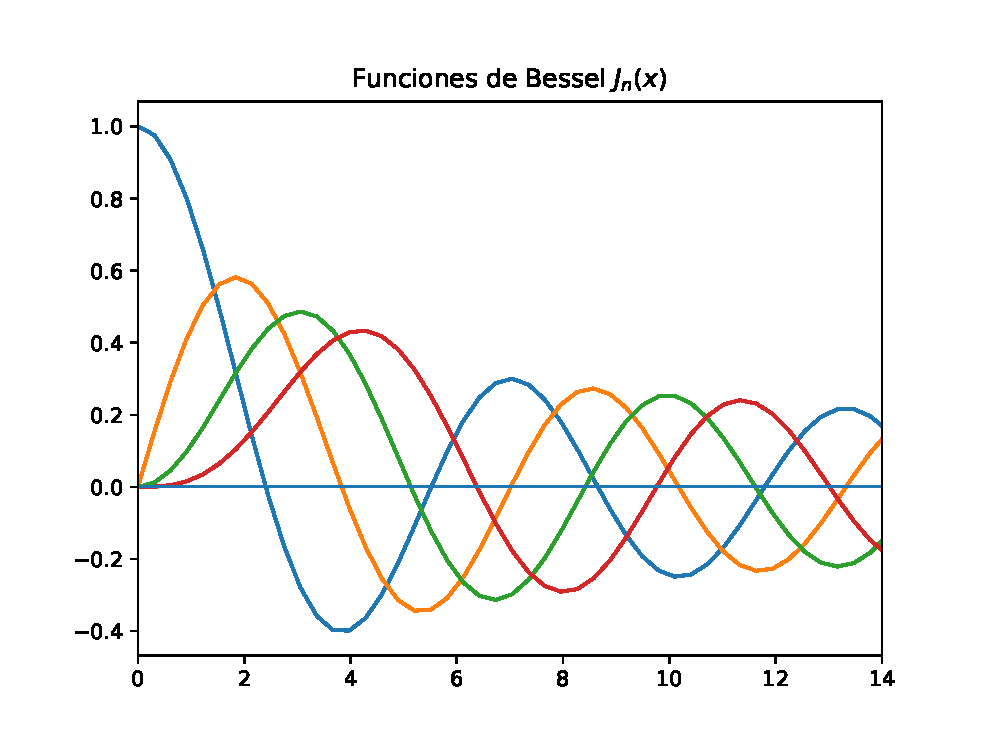
\includegraphics[scale=0.57]{Imagenes/plot_Bessel.eps}
\end{figure}
\end{frame}
\begin{frame}
\frametitle{Base completa}
Entenderemos una base completa como aquella que permite expresar a una función cualquiera en términos de otras funciones, en nuestro caso, funciones especiales:
\pause
\begin{align*}
f(x) = \sum_{n}^{\infty} c_{n} \, \varphi_{n}(x)
\end{align*}
\end{frame}
\begin{frame}
\frametitle{Ortogonalidad en la base}
Se debe de garantizar que las funciones que conforman la base, deben de ser ortogonales entre sí, es decir:
\pause
\begin{align*}
(\varphi_{n}, \varphi_{m}) = \int_{a}^{b} \varphi_{n}^{*} \, \varphi_{m} \dd{x} = A_{n} \, \delta_{nm}
\end{align*}
\pause
En el caso que $A = 1$, se tiene una base \emph{ortonormal}, es decir, es ortogonal y está normalizada a $1$. \pause Tendremos casos en donde la base de ciertas funciones especiales la condición de normalización no es unitaria.
\end{frame}
\begin{frame}
\frametitle{Extendiendo la ortogonalidad}
Podemos extender la condición de ortogonalidad al incluir una función de peso: $\omega(x) \in \mathbb{R}$, tal que:
\begin{eqnarray*}
(\omega \, \varphi_{n}, \varphi_{m}) &=& \int_{a}^{b} \omega(x) \, \varphi_{n}^{*}(x) \, \varphi_{m}(x) \dd{x} = A_{n} \, \delta_{nm} = \\[0.5em] \pause
&=& \delta_{nm} \int_{a}^{b} \omega (x) \, \abs{\varphi(x)}^{2} \dd{x} = \\[0.5em] \pause
&=& (\omega \, \varphi_{n}, \varphi_{m}) = \\[0.5em] \pause
&=& A_{n} \delta_{nm}
\end{eqnarray*}
\end{frame}
\begin{frame}
\frametitle{Cuando no se da la ortogonalidad}
En el caso en que tengamos que las funciones que conforman a la base no son ortogonales entre sí, es posible obtener la condición de ortogonalidad.
\\
\bigskip
\pause
Para ello usamos la \emph{técnica de ortogonalización de Gram-Schmidt}.
\end{frame}

\subsection{Propiedades de las funciones especiales}

\begin{frame}
\frametitle{Propiedades generales}
Cada una de las funciones especiales enlistadas cuenta con un conjunto de propiedades que las caracterizan.
\\
\bigskip
\pause
La obtención de estas propiedades se recupera tanto de las soluciones de la EDO2H, así como de las CDF, las CI, y de la base completa que forman las soluciones.
\end{frame}
\begin{frame}
\frametitle{Expresión de las funciones especiales}
Cada función especial tendrá una expresión que podemos evaluar a partir del orden\footnote{Dependiendo del texto que se consulte, puede variar el nombre del orden, en algunos textos se indica el orden $\nu$ de la función de Bessel.} $n$ que se indique, \pause en el caso de las funciones de Bessel:
\begin{align}
\setlength{\fboxsep}{3\fboxsep}\boxed{
J_{n} (x) = \sum_{n=0}^{\infty} \dfrac{(-1)^{n}}{n! \, \Gamma (n + p + 1)} \left( \dfrac{x}{2} \right)^{n+2p}}
\label{eq:ecuacion_08_06}
\end{align}    
\end{frame}
\begin{frame}
\frametitle{Condición de ortogonalización}
En algunas funciones especiales la condición de ortogonalización se revisa con funciones del mismo orden, pero variando un parámetro en el argumento:
\pause
\begin{align*}
\int_{0}^{1} x \, J_{n}(k_{m} \, x) \, J_{n}(k_{l} \, x) \dd{x} = \begin{cases}
0 & m \neq l \\
\dfrac{1}{2} \, J_{n+1}^{2} (k_{m}) & m = l
\end{cases}
\end{align*}
\pause
En este caso, se tiene la condición de ortogonalidad pero la normalización no es unitaria.
\end{frame}
\begin{frame}
\frametitle{Función generatriz}
Las funciones de Bessel de orden entero tienen una función generatriz, es decir, existe una función $g(x, t)$, tal que:
\pause
\begin{equation}
g (x, t) = \sum_{n=-\infty}^{\infty} t^{n} \, J_{n} (x)
\label{eq:ecuacion_27_25}
\end{equation}
\pause
en donde hay que determinar la función $g (x, t)$
\end{frame}
\begin{frame}
\frametitle{Función generatriz}
Haciendo el respectivo procedimiento en donde se ocupa la definición de la función especial, se llega a:
\begin{equation}
g (x, t) = \exp \left[ \dfrac{x}{2} \left( t - \dfrac{1}{t} \right) \right] = \sum_{n=-\infty}^{\infty} t^{n} \, J_{n} (x)
\label{eq:ecuacion_27_27}
\end{equation}
\end{frame}
\begin{frame}
\frametitle{Fórmula de Rodrigues}
Dada una función de peso $\omega(x) > 0$, se definen las funciones:
\pause
\begin{align*}
\phi_{n} = \dfrac{1}{\omega(x)} \, \dv[n]{x} \big[ x^{n} \, \omega(x) \big]
\end{align*}
a esta expresión se le conoce como \emph{fórmula de Rodrigues}. \pause En el caso particular para las funciones de Bessel, no se cuenta con una fórmula de Rodrigues, para las demás funciones especiales si se tiene esta expresión.
\end{frame}
\begin{frame}
\frametitle{Relaciones de recurrencia}
A partir de la definición de la función especial, es posible construir una serie de relaciones de recurrencia:
\begin{align*}
J_{m-1} (x) + J_{m+1} (x) &= \dfrac{2 \, m}{x} \, J_{m} (x) \\[0.5em]
J_{m-1} (x) - J_{m+1} (x) &= 2 \, J_{m}^{\prime} (x) \\[0.5em]
J_{m-1}(x) &= \dfrac{m}{x} \, J_{m} (x) + J_{m}^{\prime} (x) \\[0.5em]
J_{m+1}(x) &= \dfrac{m}{x} \, J_{m} (x) - J_{m}^{\prime} (x)
\end{align*}
\end{frame}
\begin{frame}
\frametitle{Relaciones de recurrencia}
Las relaciones de recurrencia permiten obtener las expresiones de una función especial de orden $n + 1$ a partir de las expresiones de orden $n$ y $n - 1$, como en en el ejemplo anterior.
\pause
\\
\bigskip
En algunas relaciones de recurrencia se ocupa el valor de la derivada de la función especial para obtener otra expresión.
\end{frame}
\begin{frame}
\frametitle{Paridad de las funciones especiales}
Es posible evaluar una función especial con un argumento negativo y obtener la expresión en términos de la misma función especial evaluada con el argumento positivo y un factor de signo:
\pause
\begin{align*}
J_{-n} (x) = (-1)^{n} \, J_{n}(x)
\end{align*}
\end{frame}
\begin{frame}
\frametitle{Aplicaciones}
El siguiente paso luego de haber obtenido las propiedades de cada función especial, es resolver problemas similares a los que se plantearon en un inicio.
\\
\bigskip
De tal manera que ya no será necesario obtener las expresiones nuevamente, sino más bien, ocupar los resultados.
\end{frame}
\begin{frame}
\frametitle{Distribución de temperatura en un cilindro}
Veamos el siguiente ejemplo: \pause Considera un cilindro largo macizo de radio $r = a$ cuya superficie lateral se mantiene a temperatura cero.
\\
\bigskip
\pause
Inicialmente, la temperatura en el cilindro está dada por $f(r)$. \pause Suponiendo que no hay variación con respecto al eje $z$ y que la temperatura para cada radio $r$ es la misma para toda esa superficie (independiente de $\theta$). \pause \textbf{Describe la distribución de temperaturas $u(r, t)$ en el cilindro}.
\end{frame}


\end{document}